% !TEX root = saveliev_physics_general_course_2.tex
%!TEX TS-program = pdflatex
%!TEX encoding = UTF-8 Unicode


\chapter[CÁC PHƯƠNG TRÌNH MAXWELL]{CÁC PHƯƠNG TRÌNH MAXWELL}\label{chap:9}
\chaptermark{CÁC PHƯƠNG TRÌNH MAXWELL}

\section{Điện trường xoáy}\label{sec:9_1}

Xét suất điện động trên một vòng dây tĩnh mang dòng điện, và từ thông biến thiên do biến thiên từ trường.
Việc có dòng điện cảm ứng cho thấy sự biến thiên từ trường sinh ra các ngoại lực trong vòng dây tác dụng lên các hạt tải điện.
Các ngoại lực này không thể liên quan tới các quá trình hóa hoặc nhiệt trong vòng dây, càng không thể do lực từ do lực từ không sinh công trên hạt tích điện.
Sử dụng loại trừ, ta được dòng cảm ứng là do điện trường bên trong vòng dây.
Đặt $\vec{E}_B$ là độ lớn của trường này (ký hiệu này, cũng như $\vec{E}_q$ dưới đây, được dùng tạm và ta sẽ bỏ ký tự dưới $B$ và $q$ sau).
Suất điện động bằng lưu số vector $\vec{E}_B$ dọc vòng dây:
\begin{equation}\label{eq:9_1}
    \ab{\mathcal{E}}{i} = \oint \vec{E}_B \ccdot \derivec{l}.
\end{equation}

Thế vào \eqn{9_1} $\ab{\mathcal{E}}{i} = -\diffin{\Phi}{t}$ cho $\ab{\mathcal{E}}{i}$ và biểu thức $\int\vec{B}\ccdot\derivec{S}$ cho $\Phi$, ta có
\begin{equation*}
    \oint \vec{E}_B \ccdot \derivec{l} = -\diff{}{t} \int_S \vec{B} \ccdot \derivec{S}
\end{equation*}

\noindent
(tích phân bên phải được lấy trên bất kỳ mặt nào có biên nằm trên vòng kín).
Do vòng kín và mặt được chọn không đổi theo thời gian, có thể đảo phép đạo hàm thời gian và tích phân mặt:
\vspace{-12pt}
\begin{equation}\label{eq:9_2}
    \oint \vec{E}_B \ccdot \derivec{l} =  - \int_S \diffpartial{\vec{B}}{t} \ccdot \derivec{S}.
\end{equation}

\noindent
Do vector $\vec{B}$ phụ thuộc vào, một cách tổng quát, cả thời gian và tọa độ, ta phải đặt phép đạo hàm riêng theo thời gian vào bên trong tích phân (tích phân $\int\vec{B}\ccdot\derivec{S}$ là một hàm của thời gian).

Biến đổi vế trái của \eqn{9_2} dùng định lý Stokes:
\begin{equation*}
    \int_S (\curlop{\vec{E}_B}) \ccdot \derivec{S} = - \int_S \diffpartial{\vec{B}}{t} \ccdot \derivec{S}.
\end{equation*}

\noindent
Do mặt được chọn là ngẫu nhiên, ta phải có biểu thức sau
\begin{equation}\label{eq:9_3}
    \curlop{\vec{E}_B} = - \diffpartial{\vec{B}}{t}.
\end{equation}

\noindent
Curl của trường $\vec{E}_B$ tại mọi điểm trong không gian bằng ngược dấu đọa hàm của vector $\vec{B}$.

Nhà vật lý người Anh James Maxwell cho rằng từ trường biến thiên theo thời gian sinh ra trường $\vec{E}_B$ cho dù có hay không một vòng dây trong không gian.
Sự hiện diện của vòng dây chỉ giúp phát hiện ra điện trường tại các điểm tương ứng trong không gian do dòng điện cảm ứng trong cuộn dây.

Do đó, theo Maxwell, \textit{một từ trường biến thiên theo thời gian sinh ra điện trường}.
Trường này $\vec{E}_B$ khác biệt hẳn so với trường tĩnh điện $\vec{E}_q$ sinh ra bởi điện tích đứng yên.
Trường tĩnh điện là trường thế, các đường sức bắt đầu và kết thúc tại các điện tích.
Curl của vector $\vec{E}_q$ bằng 0 tại mọi điểm:
\begin{equation}\label{eq:9_4}
    \curlop{\vec{E}_q} = 0
\end{equation}

\noindent
[see \eqn{1_112}].
Theo \eqn{9_3}, curl của $\vec{E}_B$ khác không.
Do đó, trường $\vec{E}_B$ giống từ trường khi đều là trường xoáy
Các đường sức của $\vec{E}_B$ được khép kín.

Do đó một điện trường có thể là trường thế ($\vec{E}_q$) hoặc trường xoáy ($\vec{E}_B$).
Trong trường hợp tổng quát, điện trường có thể gồm thành phần $\vec{E}_q$ sinh ra bởi điện tích và thành phần $\vec{E}_B$ sinh ra bởi từ trường biến thiên theo thời gian.
Cộng \eqns{9_3}{9_4}, ta có curl của điện trường tổng hợp $\vec{E}=\vec{E}_B+\vec{E}_B$:
\begin{equation}\label{eq:9_5}
    \curlop{\vec{E}} = - \diffpartial{\vec{B}}{t}.
\end{equation}

\noindent
Đây là một công thức nền tảng trong lý thuyết điện từ Maxwell.

Sự tồn tại mối liên hệ giữa từ trường và điện trường [biểu diễn như ở \eqn{9_5}] là một lý do tại sao tính toán riêng rẽ các trường này chỉ mang tính tương đối.
Một điện trường được thiết lập bởi hệ các điện tích đứng yên.
Nếu các điện tích này đứng yên tương đối so với một hệ quy chiếu quán tính nào đó, khi này chúng sẽ di chuyển so với một hệ quy chiếu quán tính khác, và do đó thiết lập nên không chỉ điện trường mà còn từ trường.
Một đoạn dây thẳng mang dòng điện không đổi sinh ra từ trường không đổi tại mọi điểm trong không gian.
Mặt khác, đoạn dây này di chuyển trong các hệ quy chiếu quán tính khác.
Do đó , từ trường mà nó gây ra tại tọa độ $x$, $y$, $z$ cho trước sẽ thay đổi, và do đó sinh ra một điện trường xoáy.
Do đó, một trường "thuần túy" điện trường hoặc từ trường so với một HQC quán tính nào đó sẽ là hỗn hợp của điện trường và từ trường, hình thành một điện từ trường so với các HQC khác.

\section{Dòng điện dịch}\label{sec:9_2}

Với một điện từ trường tĩnh (\ie không thay đổi theo thời gian), curl của vector $\vec{H}$ cho bởi \eqn{7_9} bằng mật độ dòng cục bộ:
\begin{equation*}
    \curlop{\vec{H}} = \vec{j}.
\end{equation*}

\noindent
Vector $\vec{j}$ liên hệ với mật độ điện tích bởi định luật bảo toàn điện tích \eqref{eq:5_11}:
\begin{equation*}
    \divop{\vec{j}} = - \diffpartial{\rho}{t}.
\end{equation*}

Một điện từ trường chỉ tĩnh chỉ khi mật độ điện tích $\rho$và mật độ dòng $j$không phụ thuộc thời gian.
Trong trường hợp này, theo  \eqn{5_11}, div của $\vec{j}$ bằng không.
Do đó, các đường dòng (đường của vector $\vec{j}$) không có điểm nguồn và khép kín.

Ta hãy xem xét liệu \eqn{7_9} có đúng với trường biến thiên theo thời gian.
Xét dòng điện khi một tụ điện được nạp từ một nguồn điện áp không đổi $U$.
Dòng điện biến thiên theo thời gian (dòng ngừng khi điện thế trên tụ bằng $U$).
Các đường dòng bị ngắt tại không gian giữa các bản tụ (\fig{9_1}; các đường dòng biên trong bản được cho bởi đường nét đứt).

\begin{figure}[t]
	\begin{center}
		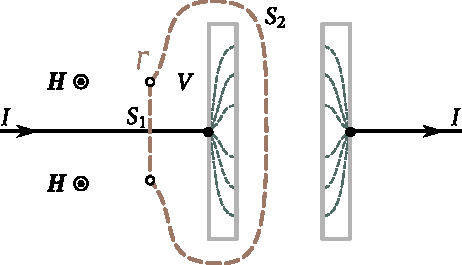
\includegraphics[scale=1]{figures/ch_09/fig_9_1.pdf}
		\caption[]{}
		\label{fig:9_1}
	\end{center}
	\vspace{-0.8cm}
\end{figure}

Chọn một đường tròn kín $\Gamma$ chắn đoạn dây mà dòng chạy về phía bản tụ và tích phân  \eqn{7_9} trên mặt $S_1$ chắn bởi đường kín và cắt dây dẫn:
\begin{equation*}
    \int_{S_1} \curlop{\vec{H}} \ccdot \derivec{S} = \int_{S_1} \vec{j} \ccdot \derivec{S}.
\end{equation*}

\noindent
Biến đổi vế trái theo định luật Stokes ta được thông lượng của vector $\vec{H}$ trên vòng $\Gamma$:
\begin{equation}\label{eq:9_6}
    \oint_{\Gamma} \vec{H} \ccdot \derivec{l} = \int_{S_1} \vec{j} \ccdot \derivec{S} = I
\end{equation}

\noindent
($I$ là dòng nạp tụ).
Áp dụng tương tự cho mặt $S_2$ không cắt đoạn dây mang dòng điện (see \fig{9_1}), ta đi đến kết luận sai nghiễm nhiên như sau:
\begin{equation}\label{eq:9_7}
    \oint_{\Gamma} \vec{H} \ccdot \derivec{l} = \int_{S_2} \vec{j} \ccdot \derivec{S} = 0.
\end{equation}

\noindent
Kết quả ta nhận được cho thấy rằng với trường biến thiên \eqn{7_9} không còn chính xác.
Kết quả này cho thấy rằng phương trình của ta thiếu thành phần phụ thuộc vào đạo hàm của trường.
Với các trường tĩnh, đạo hàm này bằng 0.

Việc \eqn{7_9} không đúng với các trường không tĩnh có thể phát hiện bởi lý luận như sau.
Lấy div hai vế của \eqn{7_9}:
\begin{equation*}
    \divop{(\curlop{\vec{H}})} = \divop{\vec{j}}.
\end{equation*}

\noindent
Div của một curl luôn phải bằng không [see \eqn{1_106}].
Do đó ta có kết quả div của vector  $\vec{j}$ phải luôn bằng không.
Nhưng kết luận này trái với phương trình liên tục \eqref{eq:5_11}.
Một cách tổng quát, trong các quá trình không tĩnh, $\rho$ có thể biến thiên theo thời gian (cụ thể trong trường hợp này là mật độ điện tích trên bản tụ được tích điện).
Theo \eqn{5_11}, div $\vec{j}$ khác không.

Để tạo sự gắn kết cho \eqns{5_11}{7_9}, Maxwell đưa thêm một số hạng vào vế phải của \eqn{7_9}.
Số hạng này, lẽ dĩ nhiên có thứ nguyên của mật độ dòng.
Maxwell gọi nó là mật độ dòng điện dịch.
Do đó, theo Maxwell, \eqn{7_9} sẽ có dạng
form
\begin{equation}\label{eq:9_8}
    \curlop{\vec{H}} = \vec{j} + \ab{\vec{j}}{d}.
\end{equation}

Tổng của dòng điện dẫn và dòng điện dịch thường được gọi là \textbf{dòng điện tổng}.
Mật độ dòng tổng là
\begin{equation}\label{eq:9_9}
    \ab{\vec{j}}{tot} = \vec{j} + \ab{\vec{j}}{d}.
\end{equation}

Nếu ta giả sử rằng div của dòng điện dịch bằng dòng điện dẫn nhưng trái dấu:
\begin{equation}\label{eq:9_10}
    \divop{\ab{\vec{j}}{d}} = - \divop{\vec{j}},
\end{equation}

\noindent
thì div của vế phải \eqn{9_8}, cũng như vế trái, luôn bằng không.

Thế $\diffinpartial{\rho}{t}$ bằng $\divop{\vec{j}}$ tại \eqn{9_10} theo \eqn{5_11}, ta có biểu thức cho div của dòng điện dịch
\begin{equation}\label{eq:9_11}
    \divop{\ab{\vec{j}}{d}} = \diffinpartial{\rho}{t}.
\end{equation}

\noindent
Để liên hẹ dòng điện dịch với các đại lượng đặc trưng cho điện tích trong điện trường biến thiên theo thời gian, hãy sử dụng \eqn{2_23} mà theo đó div của vector điện dịch bằng mật độ khối điện tích tự do:
\begin{equation*}
    \divop{\vec{D}} = \rho.
\end{equation*}

\noindent
Đạo hàm theo thời gian của phương trình này
\begin{equation*}
    \diffpartial{}{t} (\divop{\vec{D}}) = \diffpartial{\rho}{t}.
\end{equation*}

\noindent

Đảo thứ tự đạo hàm theo thời gian và theo tọa độ ở vế trái.
Ta nhận được biểu thức cho đạo hàm của $\rho$ theo $t$:
\begin{equation*}
    \diffpartial{\rho}{t} = \divop{\parenthesis{ \diffpartial{\vec{D}}{t} }}.
\end{equation*}

\noindent
Thế biểu thức này vào \eqn{9_11} có
\begin{equation*}
    \divop{\ab{\vec{j}}{d}} = \divop{\parenthesis{ \diffpartial{\vec{D}}{t} }}.
\end{equation*}

\noindent
Hay
\begin{equation}\label{eq:9_12}
    \ab{\vec{j}}{d} = \diffpartial{\vec{D}}{t}.
\end{equation}

Thế \eqn{9_12} vào \eqn{9_8}, ta nhận được phương trình
\begin{equation}\label{eq:9_13}
    \curlop{\vec{H}} = \vec{j} + \diffpartial{\vec{D}}{t},
\end{equation}

\noindent
mà cũng như \eqn{9_5} là một trong các phương trình nền tảng của lý thuyết Maxwell

Ta phải nhận định rõ rằng thuật ngữ ``dòng điện dịch'' hoàn toàn đưa ra để tiện lợi cho tính toán.
Về bản chất, dòng điện dịch là một điện trường biến thiên theo thời gian.
Lý do duy nhất ta gọi đại lượng này trong \eqn{9_12} là ``dòng điện'' chỉ là thứ nguyên của địa lượng này trùng với mật độ dòng.
Trong tất cả tính chất vật lý của một dòng điện thực, dòng điện dịch chỉ có một trong đó--khả năng sinh ra từ trường.

Việc sinh ra ``dòng điện dịch'' tại \eqn{9_12} đưa ra sự đối xứng bình đnăgr cho điện trường và từ trường.
Từ hiện tượng cảm ứng điện từ ta tìm được rằng từ trường biến thiên sinh ra điện trường.
Từ \eqn{9_13} tìm được rằng một điện trường biến thiên sinh ra từ trường.

Dòng điện dịch tồn tại ở mọi nơi có điện trường biến thiên.
Cụ thể hơn, nó cũng tồn tại trong vật dẫn mang dòng điện xoay chiều.
Mặc dù vậy, dòng điện dịch trong lòng vật dẫn thông thường bỏ qua được khi so với dòng điện dẫn.

Ta nhận xét rằng \eqn{9_6} là công thức sơ bộ.
Để chặt chẽ, ta phải thêm vào vế phải thành phần dòng điện dịch do điện trường nhỏ trong lân cận mặt $S_1$.

Ta chứng minh rằng tích phân mặt tại vế phải \eqn{9_8} có cùng một giá trị với các mặt $S_1$ and $S_2$ (xem \fig{9_1}).
Cả dòng điện dẫn và dòng điện dịch do điện trường bên ngoài tụ ``chảy'' qua mặt $S_1$.
Do đó, với mặt đầu tiên
\begin{equation*}
    \text{Int}_1 = \int_{S_1} \vec{j} \ccdot \derivec{S} + \diff{}{t} \int_{S_1} \vec{D} \ccdot \derivec{S} = I + \diff{}{t} \ab{\Phi}{$1$,in}
\end{equation*}

\noindent
(ta đã thay thứ tự đạo hàm theo thời gian và theo tọa độ ở số hạng thứ hai).
Đại lượng ký hiệu $I$ là dòng điện chạy vào vật dẫn vào bản tụ bên tay trái,  $\ab{\Phi}{$1$,in}$ là thông lượng vector $\vec{D}$ chạy vào thể tích $V$ bao bởi mặt $S_1$ và $S_2$ (xem \fig{9_1}).

Với mặt thứ hai, $\vec{j}=0$, cho nên
\begin{equation*}
    \text{Int}_2 = \diff{}{t} \int_{S_2} \vec{D} \ccdot \derivec{S} = \diff{}{t} \ab{\Phi}{$2$,out}
\end{equation*}

\noindent
với $\ab{\Phi}{$2$,out}$ là thông lượng vector  $\vec{D}$ chạy ra khỏi $V$ qua mặt $S_2$.

Hiệu của hai tích phân này là
\begin{equation*}
    \text{Int}_2 - \text{Int}_1 = \diff{}{t} \ab{\Phi}{$2$,out} - \diff{}{t} \ab{\Phi}{$1$,in} - I.
\end{equation*}

\noindent
Dòng $I$ có thể ký hiệu là $\diffin{q}{t}$, với $q$ là điện tích trên bản tụ.
Thông lượng vào trong qua mặt $S_1$ equals
thông lượng ra ngoài trên cùng mặt nhưng trái dấu.
Thế $-\ab{\Phi}{$1$,out}$ vào $\ab{\Phi}{$1$,in}$ và $\diffin{q}{t}$ cho $I$, ta có
\begin{equation}\label{eq:9_14}
    \text{Int}_2 - \text{Int}_1 = \diff{}{t} \parenthesis{\ab{\Phi}{$2$,out} + \ab{\Phi}{$1$,out}} - \diff{q}{t} = \diff{}{t} \parenthesis{\Phi_D - q},
\end{equation}

\noindent
với $\Phi_D$ là thông lượng của vector $\vec{D}$ qua mặt kín hợp bởi mặt $S_1$ và $S_2$.
Theo \eqn{2_25}, thông lượng này phải bằng điện tích bên trong mặt.
Trong trường hợp này, nó chính là điện tích $q$ trên bản tụ.
Do đó, vế phải của \eqn{9_14} bằng không.
Từ đó độ lớn của tích phân mặt mật độ dòng điện tổng không phụ thuộc vào cách chọn mặt để tích phân.

có thể dựng các đường dòng cho dòng điện dịch giống như với dòng điện dẫn.
Theo \eqn{2_35}, độ điện dịch trong không gian giữa hai bản tụ bằng mật độ điện tích trên một bản: $D=\sigma$.
Do đó,
\begin{equation*}
    \dot{D} = \dot{\sigma}.
\end{equation*}

\noindent
Vế trái của công thức trên cho ta mật độ dòng điện dịch trong không gian giữa hai bản tụ, còn vế phải là mật độ dòng điện dẫn tại không gian giữa hai bản.
Sự đồng nhất của hai đại lượng này thể hiện rằng đường dòng của dòng điện dẫn chuyển thành đường dòng của dòng điện dịch tại biên của các bản tụ mà không bị ngắt quãng.
Do đó, đường dòng của dòng điện tổng là khép kín.

\section{Các phương trình Maxwell}\label{sec:9_3}

Việc tìm ra dòng điện dịch cho phép Maxwell đưa ra một lý thuyết tổng quát duy nhất cho các hiện tượng điện và từ.
Lý thuyết này giải thích toàn bộ các kết quả thực nghiệm tại thời điểm này và dự đoán các hiện tượng mới, mà sẽ được kiểm chứng về sau.
Hệ quả chính của lý thuyết Maxwell là kết luận về sự tồn tại của sóng điện từ truyền với tốc độ ánh sáng.
Nghiên cứu lý thuyết tính chất của các sóng này dẫn Maxwell dến lý thuyết điện từ của ánh sáng.

Lý thuyết này dựa trên \textbf{các phương trình Maxwell}.
Các phương trình này đóng vai trò tương đương trong điện từ học như các định luật Newton trong cơ học hoặc các định luật cơ bản của nhiệt động lực học.

\textbf{Cặp phương trình Maxwell đầu tiên} bao gồm \eqns{9_5}{7_3}:
\begin{align}
    \curlop{\vec{E}} &= - \diffpartial{\vec{B}}{t},\label{eq:9_5rev} \tag{9.5}\\
    \divop{\vec{B}} &= 0.\label{eq:7_3rev} \tag{7.3}
\end{align}

\noindent
Phương trình đầu liên hệ giá trị của $\vec{E}$ đến sự thay đổi của vector $\vec{B}$ theo thời gian và là một cách biểu diễn của định luật cảm ứng điện từ
Phương trình thứ hai chỉ ra sự không tồn tại của nguồn từ trường, \ie, từ tích.

\textbf{Cặp phương trình Maxwell thứ hai} bao gồm \eqns{9_13}{2_23}:
\begin{align*}
    \curlop{\vec{H}} &= \vec{j} + \diffpartial{\vec{D}}{t},\label{eq:9_13rev} \tag{9.13}\\
    \divop{\vec{D}} &= \rho.\label{eq:2_23rev} \tag{2.23}
\end{align*}

\noindent
Phương trình đầu thiết lập mối quan hệ giữa dòng điện dẫn và dòng điện dịch với từ trường chúng sinh ra.
Phương trình thứ hai chỉ ra rằng điện tích tự do là nguồn của vector $\vec{D}$.
Phương trình \eqref{eq:9_5rev}, \eqref{eq:7_3rev}, \eqref{eq:9_13rev} và \eqref{eq:2_23rev} là các phương trình Maxwell ở dạng vi phân.
Chúng ta chú ý rằng cặp đầu tiên chỉ gồm các tính chất đặc trưng của trường, cụ thể là $\vec{E}$ và $\vec{B}$.
Cặp thứ hai chỉ bao gồm các đại lượng phụ $\vec{D}$ và $\vec{H}$.

Mỗi phương trình vector \eqref{eq:9_5rev} và \eqref{eq:9_13rev} tương đương với ba phương trình vô hướng liên hệ các thành phần vector ở vế trái và phải.
Với phương trình \eqref{eq:1_81} và \eqref{eq:1_92}-\eqref{eq:1_91}, ta biểu diễn các phương trình Maxwell dạng vô hướng:
\begin{align}
    & \begin{cases}
        &\!\!\!\! \diffpartial{E_z}{y} - \diffpartial{E_y}{z} = - \diffpartial{B_x}{t}\\[8pt]
        &\!\!\!\! \diffpartial{E_x}{z} - \diffpartial{E_z}{x} = - \diffpartial{B_y}{t}\\[8pt]
        &\!\!\!\! \diffpartial{E_y}{x} - \diffpartial{E_x}{y} = - \diffpartial{B_z}{t}\\
    \end{cases}\label{eq:9_15}\\[5pt]
    & \quad\,\diffpartial{B_x}{x} + \diffpartial{B_y}{y} + \diffpartial{B_z}{z} = 0,\label{eq:9_16}
\end{align}

\noindent
(cặp phương trình đầu tiên),
\begin{align}
    & \begin{cases}
        &\!\!\!\! \diffpartial{H_z}{y} - \diffpartial{H_y}{z} = j_x + \diffpartial{D_x}{t}\\[8pt]
        &\!\!\!\! \diffpartial{H_x}{z} - \diffpartial{H_z}{x} = j_y + \diffpartial{D_y}{t}\\[8pt]
        &\!\!\!\! \diffpartial{H_y}{x} - \diffpartial{H_x}{y} = j_z + \diffpartial{D_z}{t}
    \end{cases}\label{eq:9_17}\\[5pt]
    & \quad\,\diffpartial{D_x}{x} + \diffpartial{D_y}{y} + \diffpartial{D_z}{z} = \rho,\label{eq:9_18}
\end{align}

\noindent
(cặp phương trình thứ hai).

Ta có tổng cộng $8$ phương trình gồm $12$ hàm là ẩn (ba thành phần của từng vector $\vec{E}$, $\vec{B}$, $\vec{D}$, $\vec{H}$.
Do số phương trình ít hơn số ẩn, \eqref{eq:9_5rev}, \eqref{eq:7_3rev}, \eqref{eq:9_13rev} và \eqref{eq:2_23rev} là chưa đủ để tìm các trường theo phân bố điện tích và dòng điện cho trước.
Để tính các trường, ta cần phương trình liên hệ $\vec{D}$ và $\vec{j}$ với $\vec{E}$ và $\vec{H}$ và $\vec{B}$ vào hệ phương trình này.
Chúng có dạng sau
\begin{align}
    \vec{D} &= \varepsilon_0\varepsilon \vec{E}, \label{eq:2_21rev}\tag{2.21}\\
    \vec{B} &= \mu_0\mu \vec{H}, \label{eq:7_17rev}\tag{7.17}
    % \vec{j} &= \sigma \vec{E}. \label{eq:5_22rev}\tag{5:22}
\end{align}
\begin{equation}\label{eq:5_22rev}
    \vec{j} = \sigma \vec{E}. \tag{5.22}
\end{equation}

Hệ các phương trình \eqref{eq:9_5rev}, \eqref{eq:7_3rev}, \eqref{eq:9_13rev} và \eqref{eq:2_23rev}, và \eqref{eq:2_21rev},
\eqref{eq:7_17rev}, \eqref{eq:5_22rev} là nền tảng cho điện động lực học cho môi trường tĩnh

Các phương trình
\begin{align}
    \oint_{\Gamma} \vec{E} \ccdot \derivec{l} &= - \diff{}{} \int_S \vec{B} \ccdot \derivec{S}, \label{eq:9_19}\\
    \oint_S \vec{B} \ccdot \derivec{S} &= 0, \label{eq:9_20}
\end{align}

\noindent
(cặp thứ nhất) và
\begin{align}
    \oint_{\Gamma} \vec{H} \ccdot \derivec{l} &= \int_S \vec{j} \ccdot \derivec{S} + \diff{}{} \int_S \vec{B} \ccdot \derivec{S}, \label{eq:9_21}\\
    \oint_S \vec{D} \ccdot \derivec{S} &= \int_V \rho\, \deriv{V}, \label{eq:9_22}
\end{align}

\noindent
(cặp thứ hai) được gọi là \textbf{Các phương trình Maxwell dạng tích phân}.

Phương trình \eqref{eq:9_19} nhận được khi lấy tích phân \eqn{9_5} trên mặt $S$ bất kỳ và biến đổi vế trái dựa theo định lý Stokes thành tích phân vòng kín $\Gamma$ là biên của mặt $S$.
Ta suy được phương trình \eqref{eq:9_21} tương tự \eqn{9_13}.
Phương trình \eqref{eq:9_20} và \eqref{eq:9_22} thu được từ \eqns{7_3}{2_23} bằng cách tích phân trên thể tích $V$ bất kỳ với phép biến đổi vế trái theo định lý Ostrogradsky-Gauss thành tích phân trên mặt kín $S$ bao quanh thể tích $V$.